\chapter{Discussion}
\label{ch:discussion}
Chapter 4, 5 and 6 introduce different methods to create a decision-making agent for navigating through intersections using deep Q-learning, while considering the uncertainty of its own decisions and the prediction of the other drivers intentions. This chapter highlights some differences and synergies of the different methods. 

\section{Guaranteeing safety}
\label{ch:system_architecture}
Safety is the most important factor of a \gls{ad} system, but since \gls{rl} is a data driven approach it is very difficult to guarantee safety in the same way e.g., a \gls{mpc} can. Safety validation in a data driven approach can be very costly as it is usually done by driving many miles and showing statistical confidence in the safety metrics~\cite{koopman2016,asljung2017}, e.g., number of interventions. That is why this section will clarify where the work in this thesis would fit in by first defining a system architecture for \gls{ad}, its modules and a short summary of the ISO 26262 standard. Then, place itself within the system and motivate how safety can be guarantied. 

The architecture of an autonomous driving system can be divided into perception, planning and control~\cite{Schwarting2018,Kortenkamp2008}.
The perception module is responsible for sensing and mapping the environment with the use of sensors such as LIDARs, cameras, radars etc. The raw data from the sensors are then processed though various sensor fusion techniques to generate a representation of the environment, e.g., position, velocity of other traffic participants while also describing the road such as width and distance to the next intersection. This information is then used by the planner to create a driving strategy of how to transverse through the world. However, the information from the sensors are often noisy, with false positives and false negatives making it difficult for the planner.

Tactical planning can be divided into three categories, the proactive, active and reactive~\cite{Berntorp2018}. A proactive module would be something like a precautionary safety module that interprets the information about the environment and create constraints that is sent to the active planner, like  driveable area, allowed speeds and actions~\cite{Shiller2007}. These constraints are generated from a set of safety goals and rules, making this the first layer of protection that can ensure safety. 
The role of the active planner is to take this sets of allowed actions and prescribe the behavior of the vehicle through decisions such as drive, yield or stop. The goal of these high level decisions is to optimize metrics such as comfort, fuel consumption and time to goal. These decisions are then sent to a motion planner that generates a safe dynamically feasible path for the vehicle for a shorter planning horizon of around $0.1$s. 
At the same time, a reactive, collision avoidance, module make sure that the chosen decision and path does lead to any collisions~\cite{brannstorm2010}. Unlike the decision maker, the collision avoidance module main goal is to identify imminent danger~\cite{brannstorm2014} and therefore has access to more aggressive actions like emergency braking to ensure safety. 
 
In the industry today the main standard for functional safety in motorized vehicles is the ISO 26262 standard, titled "Road vehicles – Functional safety"~\cite{ISO26262}. It uses a \gls{asil} to classify the inherent safety risk in an automotive system and the functions or modules of such a system. The \gls{asil} classification is used to express the level of risk reduction required to prevent a specific hazard, from \gls{asil} D to \gls{asil} A. \gls{asil} D represents the highest hazard level and \gls{asil} A the lowest. There is a level with no safety relevance and only standard Quality Management processes are required, this level is referred to as QM.

\begin{figure}[h]
	\centering
	 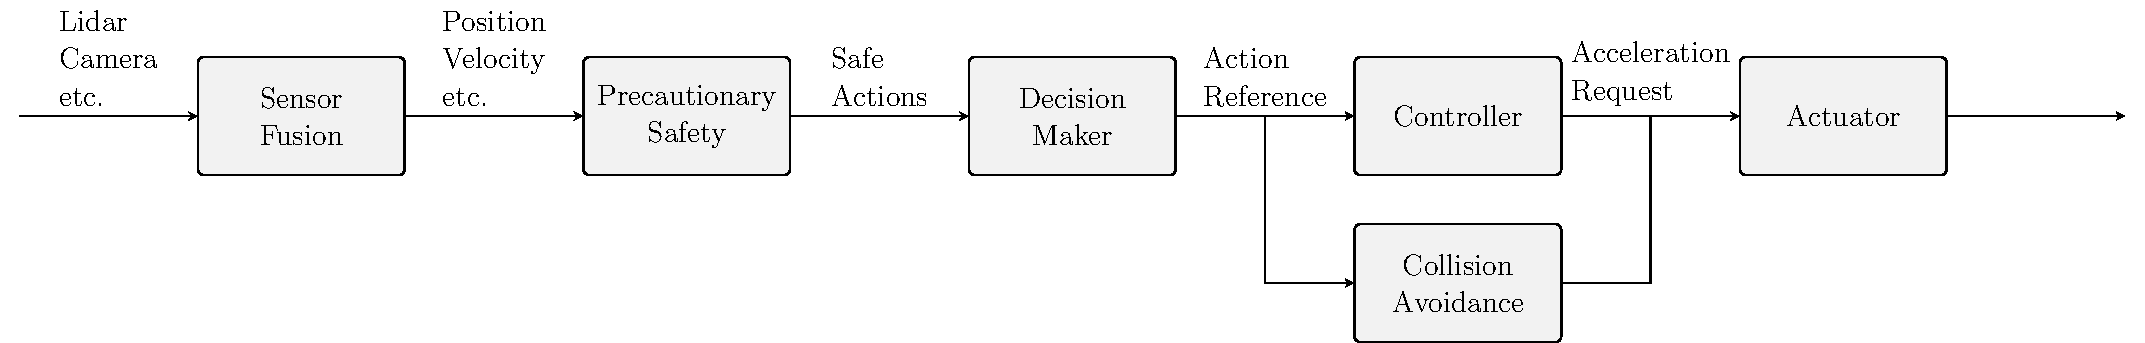
\includegraphics[width=\linewidth]{YourThesis/chapters/figures/pomdp/figures-system_architecture.pdf}
%	\begin{tikzpicture}[
%		node distance=8mm and 30mm,
%		node font= \Large,
%		box/.style = {draw, thick, rectangle, rounded corners=0.1cm, fill=gray!10, minimum width=3.5cm, minimum height=2cm, align=center},
%		sx+/.style = {xshift = 2mm},
%		sx+/.style = {xshift = 2mm}
%		]
%
%		% \node[draw,thick,rectangle,rounded corners =0.05cm,fill=gray!10,minimum width=2cm,minimum height = 2cm] (SF) at (2,0) {Sensor Fusion};
%		
%		% \draw[arrow,thick] (0,0) --(SF) node [midway,above] {Sensors: Lidar, Radar, Camera, Sonar};
%
%		% \node[draw,thick,rectangle,rounded corners =0.05cm,fill=gray!10,minimum width=2cm,minimum height = 2cm, shift={(2,0,0)}] (SF) at (2,0) {Sensor \\ Fusion};
%		
%		\node (start) at (0,0) {};
%		\node (SF) [box, right=of start.east] {Sensor \\ Fusion};
%		\node (PS) [box, right=of SF.east] {Precautionary \\ Safety};
%		\node (DM) [box, right=of PS.east] {Decision \\ Maker};
%		\node (Con) [box, right=of DM.east] {Controller};
%		\node (CA) [box, below=of Con] {Collision \\ Avoidance};
%		\node (Act) [box, right=of Con.east] {Actuator};
%		\node (end) [right=of Act] {};
%
%		\draw[arrow,thick,align=left] (start) --+(SF) node [midway,above] {Lidar\\Camera\\etc.};
%		\draw[arrow,thick,align=left] (SF) --+(PS) node [midway,above] {Position\\Velocity\\etc.};
%		\draw[arrow,thick,align=left] (PS) --+(DM) node [midway,above] {Safe\\Actions};
%		\draw[arrow,thick,align=left] (DM) --+(Con) node [midway,above] {Action\\Reference};
%		\draw[arrow,thick,align=left] (DM) -| ($(DM.east) + (1.5,0mm)$) |- (CA) node [midway,above] {};
%		\draw[arrow,thick,align=left] (CA) -| ($(CA.east) + (1.5,0mm)$) |- (Act) node [midway,above] {};
%		\draw[arrow,thick,align=left] (Con) --+(Act) node [midway,above] {Acceleration\\Request};
%		\draw[arrow,thick,align=left] (Act) --+(end) node [midway,above] {};
%	% --> Sensor Fusion --> Precautionary Safety --> |Decision Maker --> Controller |--> Actuator -->
%	% 																->Collision Avoidance |
%
%	\end{tikzpicture} 
	\caption{Representation of the system architecture.}
	\label{fig:system_architecture}
\end{figure}

Although safety is the most important requirement for enabling autonomous driving, the work in this paper does not make any safety guarantees. Instead, it is proposed that the decision-making algorithms presented in this paper be used in the system architecture shown in Figure~\ref{fig:system_architecture}. This approach allows higher \gls{asil} to be applied to the precautionary safety and collision avoidance modules, while the decision-making algorithms focus primarily on comfort. As a result, the \gls{asil} classification for the decision-making components could be at lower levels, potentially even classified as QM in the best case.

\section{Designing the reward function and terminal states}
The reward function introduced in Chapter~\ref{ch:reward_function_def} is a crucial component that significantly influences the behavior and performance of a reinforcement learning agent. By carefully designing and tweaking the reward function in \eqref{eq:thesis_reward_function}, the agent can be guided towards desirable behaviors and optimize its decision-making policy. 

The results from Chapter~\ref*{ch:modeling_intersection} and \ref{ch:uncertainty} show a collision rate of $1-3\%$, which may seem high for \glspl{av}. However, within the proposed system architecture from Figure~\ref{fig:system_architecture}, this collision rate can be interpreted as interventions by a collision avoidance system, such as emergency braking. This interpretation can be achieved by adjusting the simulation parameters, for example, increasing the size of the cars or redefining the collision state to represent a collision avoidance intervention state.

% In comparison to \paperLSTM \ and \paperMPC, the need for a terminal state was removed for \paperEnsamble \ and \paperBelief, by excluding that state transaction in the experience replay, effectively allowing the agent to continue forever. While in \paperLSTM \ there was a negative reward for choosing an action to follow a non-existing car. This could also be removed by using Q-masking in \paperMPC \ and \paperEnsamble. 


\section{Modular models in autonomous vehicles}
There are two common strategies for creating and deploying \glspl{dqn} to the real world: training a comprehensive model that encapsulates everything or training smaller, specialized models and switching between them as needed. The proposed MLEMTRL algorithm from Chapter~\ref{ch:generalize} is a step towards the latter approach of using smaller models. Combined with the uncertainty measurements in Chapter~\ref{ch:uncertainty}, instead of reverting to a default action when uncertainty is high, the agent can instead trigger a model change. MLEMTRL can then be used to determine which model to switch to, ensuring a more adaptive and robust decision-making process.

This approach allows for modularity and flexibility, enabling easier updates and maintenance since individual models can be refined or replaced without affecting the entire system. Additionally, smaller models are less likely to overfit to irrelevant details present in a larger, comprehensive dataset, leading to more generalizable and robust performance in their specific domains. They also require less computational power and memory, making them more suitable for deployment on \gls{av}s with limited resources. Smaller models are generally easier to interpret and debug, facilitating understanding of the decision-making process and identifying any issues or biases, which is an important property to have when developing \gls{av}s.

% \section{Simulation and real world}
% Bridging the gap between simulation and real world. Ever evolving driving styles. Building trust. 
% Public trust is essential for the widespread adoption of AVs. Building this trust requires addressing concerns about safety, reliability, and the overall impact of AVs on society.
% Transparency and Communication: Providing clear and transparent information about how AV systems work, their safety features, and their limitations can help in building public trust. This includes communicating the results of safety tests and real-world performance data.
% Regulatory Compliance: Ensuring that AVs meet or exceed regulatory standards for safety and performance is crucial. Collaborating with regulatory bodies to establish and adhere to stringent safety protocols can reassure the public.
% Demonstrations and Pilot Programs: Conducting public demonstrations and pilot programs can help in showcasing the capabilities and safety of AVs. Allowing people to experience AVs firsthand can alleviate fears and misconceptions.